%% Main Document
\pagestyle{plain}
\setcounter{page}{1}

%%%
\section{Introduction}\label{cha:intro}
This is the final report treating the final project in the course
TSIU03 System design. The project was to design and implement a device
used for audio signal processing. 

Using a DE2 board an external audio source can be connected via a
3.5mm port, the signal is then processed by the application and an
image is rendered on a vga screen displaying four signal level bars
representing the left and right channels both before and after
manipulation. There is also two bars displaying the current volume and
balance setting.

The application also accepts input via a ps/2 keyboard used for
setting volume  

%%%
1/2 page

{\LARGE Har du inte läst README.txt (efter 23/10), gör det omgående!}

%%%
\section{Achievements}\label{cha:achievements}
\subsection{User Noticable Achievements}\label{sec:userachievments}
\begin{itemize}
\item Remarkably astonishing graphics.
\item Power level indicators for both the input and output sound signal. 
\item The indicators are moving at a smooth rate with absolutely no flickering.
\item Displaying the current volume and balance adjustments made in a user friendly way.
\item Both the minimum and maximum level of adjustments available to the volume and balance is visible to the user.
\item A mute button is shown if the volume is set to be muted.
\item Output sound is sent to a class-D amplifier.
\item Each bar has a peak level indicator.
\item The peak level indicator falls slowly when the power bar is lower than the peak level indicator.
\end{itemize}

\subsection{Design Challenges}\label{sec:designchallenges}
\begin{itemize}
\item Use the SRAM to store information about a background picture.
\item Implement a low-pass filter for our signal level indicators. 
\item Bar graph rendering (which pixels to write/blank).
\item The logic of adjusting the volume and balance correctly.
\item Detect each key press only once to prevent drastic changes.
\end{itemize}
%%%
1/2 page

Outline the technical challenges that you have solved in your project. This is not the same as the requirements. For instance, it is not a challenge to “use the DE2 board”, it is not a challenge to “use 16 bits for the audio signal”. But it is a challenge to “generate an echo of 0.1 to 3s” or “display numbers on the screen” or “display bars for a signal level indicator on the screen”. Additionally, to have a “smooth movement of the signal level indicator bars on the screen” is an extra achievement apart from just displaying the bars. There are two tables. In the first one (Achievements) write the technical challenges that a user can notice (like the previous ones). In the second table (Design Challenges) write the challenges of the hardware design that cannot be observed from the outside. Like “use the SRAM to store both an image and audio data”, or “implement a low-pass filter with cut-off frequency 500 Hz”, or “transform the value of a sound sample into a coordinate in the screen for the oscilloscope”, or “determine the size of the memory for...”, or “codify the image in a way that uses a small amount of memory”. Note that some difficulties found during the project may not be technical challenges. Some examples are “much time spent on debugging” or “it was difficult to coordinate the group”. Please, keep these difficulties for Subsection 6, where the Project Execution is evaluated.

%%%
\section{System Level Description}\label{cha:syslvl}
\begin{figure}[H]
  \centering
  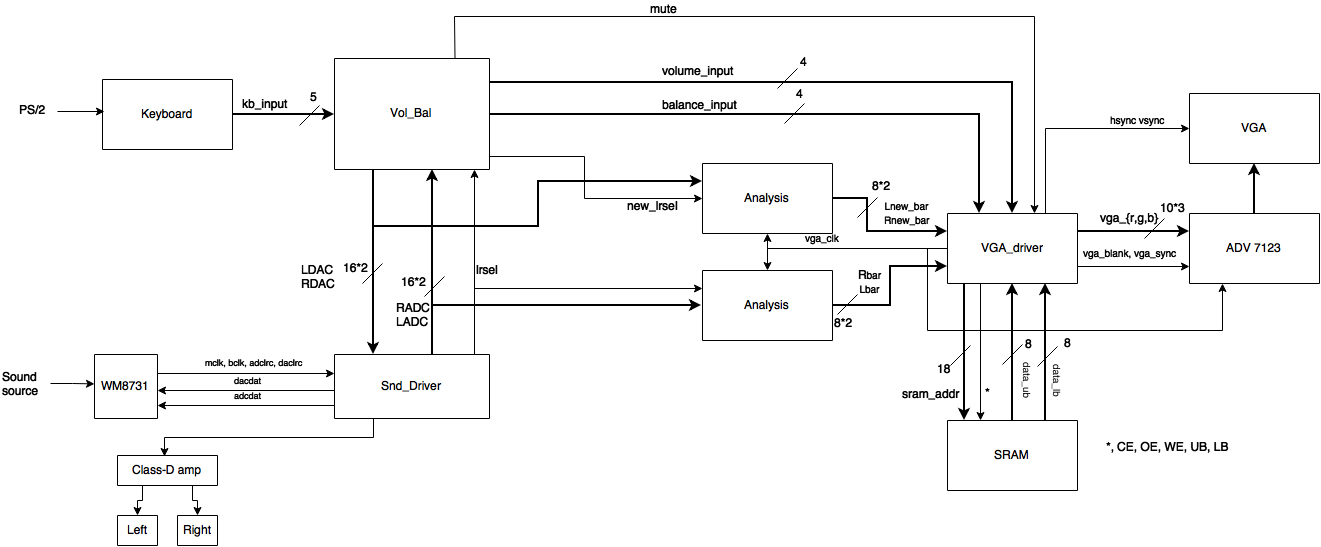
\includegraphics[width=16cm]{overview}
  \caption{G41 Project System Overview}
  \label{fig:overview}
\end{figure}

The project consists of five major modules -- \texttt{Keyboard, Vol\_Bal, Snd\_Driver, Analysis, }and \texttt{VGA\_Driver}. Presented here is an overview of the modules, and more detailed functionality is described in the \citeD.

The system takes, with help of \texttt{Snd\_Driver}, digitally encoded sound from the WM8731 chip. The sound data is passed on to the first instance of \texttt{Analysis} which provides (in order to smoothen the bar movements) low-pass filtered control signals to \texttt{VGA\_Driver:bartender} to assist the rendering of the pre-processing bar graphs done by \texttt{VGA\_Driver} as a whole. The audio data from \texttt{Snd\_Driver} is also passed on to \texttt{Vol\_Bal} which in combination with the control signals from \texttt{Keyboard} adjusts the audio balance %% mjaaa, omformuleras nog
and volume and sends it back to \texttt{Snd\_Driver} which sends signals for the class-D amplifier through the GPIO:s. The adjusted audio is also forked off to a second \texttt{Analysis} instance, which assists the post-processing bar graph rendering.

Whereas \texttt{Keyboard} and \texttt{Analysis} already are fairly small and monolithic modules, and \texttt{Snd\_Driver} and \texttt{Vol\_Bal} consists of three submodules each, \texttt{VGA\_Driver} consists of no less than twelve submodules.

\texttt{Keyboard} handles the PS/2 keyboard user input. The module filters break scan codes (F0$_{16}$, XX$_{16}$) bytewise (11 bit/byte) and compares the XX$_{16}$ byte (iff directly preceeded by F0$_{16}$) to the control key values. This approach will allow the system to respond to the regular keys (ARROW keys and END) as well as corresponding numeric keypad keys as initial E0$_{16}$ bytes are discarded. Upon a registered valid key release, a 5-bit control signal (\verb=kb_input=)is sent for a single clock cycle to \texttt{Vol\_Bal}.

\texttt{Analysis} reads the \verb=ADC= signals and lowpass filters these with a saturation time of approximately 100 ms (4096 clock cycles). These signals are converted to a graph height (in pixels) and passed on to \verb=bar_tender=.

\texttt{Snd\_Driver} have the three submodules \verb=Snd_Driver:{Ctrl,Channel_Mod}= if we count the two instances of \texttt{Channel\_Mod}. These are verbatim copies of \emph{Laboration 4}. The only difference is that the outputs are sent to GPIO pins (and from there via an i2c adapter to the class-D amp) as well as back to the WM8731 codec.

\texttt{Vol\_Bal} consists of the three submodules \verb=Vol_Bal:{Current_Vol_Bal,{Volume,Balance}_Adjustment}=. \verb=Current_Vol_Bal= reads \verb=kb_input= and updates registers representing system levels of volume, balance and mute.
\verb=Volume_Adjustment= adjusts volume according to the volume\_level input from \verb=Current_Vol_Bal=, decreasing amplitude by up to -30 dB in 3 dB decrements, and \verb=Balance_Adjustment= adjusts the audio according to system balance level, resulting in a linear scaling the incoming amplitude. The stronger a channel bias, the higher the signal reduction of the opposing channel. The affected channel loses 1/8 of the amplitude per level of bias.

\texttt{VGA\_Driver} with its submodules handles the rendering of the UI. The module is, in essence, a modified version of the module used in \emph{Laboration 3}. The most significant difference is found in the two new modules \verb=VGA_Driver:Bar_Tender= and \verb=VGA_Driver:Bar_Mixer=. \verb=Bar_Tender= uses the output from \verb=Vol_Bal= and each of the \verb=Analysis= modules along with \verb={h,v}cnt= to calculate which pixel is to be rendered and if it should be rendered from the background image or if to draw it black. The result of the calculations is the control signal \verb=render_bar=. This signal is then passed to \verb=Bar_Mixer=, which is basically a multiplexer, either forwarding the loaded background colors or a blacked out pixel depending on \verb=render_bar= from \verb=Bar_Tender=.

%%%
1 to 2 pages\\
Block diagram + description

%%%
\section{Justification of the Achievements}\label{cha:justice}
%\input{.tex/foo.tex}

%%%
4 to 6 pages

In this subsection, explain how you have solved the challenges described in Subsection 2. It is important that you show how you got from the challenge to a specific solution, and do not miss steps. From the challenge, to the algorithm (mathematical explanation or model), maybe doing some tests in Matlab to take design decisions and validate that the algorithm works. Include the mathematical equations if the algorithm is not obvious. From the algorithm to the hardware implementation, making the numbers of sizes for memories, timing for the signals, design alternatives, decision that you took and why, etc. Include relevant pictures of the circuits or sub-modules of the system to support the explanations. IMPORTANT: You can structure this subsection as a description of the sub-modules of your system, but you have to be aware that what is really important is that you explain clearly how you solved the challenges that you found.
%%%
\section{User Interface}\label{cha:ui}
The system is controlled by 5 keys on a PS/2-connected keyboard. Down in the table you can see which key that changes what in the system.


\begin{figure}[h]
\centering
%\caption{PS/2 keys and how the input affects the system.}
\begin{tabular}{|c|c|}
\hline
KEY & Function\\ \hline
U ARROW & Volume Increase\\ \hline
L ARROW & Balance Bias Left\\ \hline
D ARROW &  Volume Decrease\\ \hline
R ARROW &  Balance Bias Right\\ \hline
END		&  Mute Volume\\ \hline
\end{tabular}
\caption{PS/2 keys and how the input affects the system.}
\label{fig:scancodes}
\end{figure}


The volume level has eleven diffrent stages, exclusive mute. When the volume is at max, the whole bar will be red, and when the volume is decreased by one the bar will decrease to show the current volume.

The balance level has eighteen diffrent stages. Eight for left balance, eight for right balance and one stage when the signal is equal. When the balance is equal for left and right the only thing you will notice is the bar and divider. But when you for example press the left arrow, the left side will be filled and the outgoing volume on the right will of course decrease.

To indicate that mute is enable you can see one green speaker with a cross to the left side of the picture, and when mute is disable there will only be black. You will also be able to see that the after bars will not show anything, due that nothing is beeing sent out. 

You will be able to see one peak level indicator for each bar, the peak level indicator falls slowly when the power bar is lower than the peak level indicator. With our peak level indicator our user expreience is taken to a whole new level, as you will notice when you use our system you will be overwhelming by the effect.

\begin{figure}[h]
	\centering
        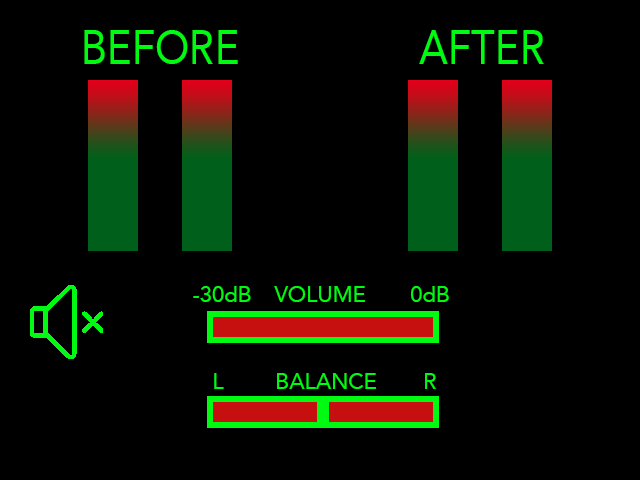
\includegraphics[scale=1]{UI2.png}
       \caption{User interface}
        \label{fig:user interface}
\end{figure}



%%%
1 page
How to control the system + image visualized on the screen

%%%
\section{Improvements}\label{cha:improvements}
The system follows the requirement and design specification quite closely. However there are still possibilities to further develop it into an enjoyable piece. There's a bug with the peak level indicator.  At certain changes, the peak level indicator will disappear and begin falling from the top of the bar, as if it had just rendered a peak that was as big  as the entity of the bar. The peak level indicator, feature wise, could when updated have a slight pause at the peak, so it can be observed more clearly before beginning to drop.

The bars of the sound amplitude are currently a gradient drawn on the background image, being covered by a black bar, to display the amplitude in a gradient bar. However, since it's drawn in the image of the background, the gradient can't change. A possible improvement to the aesthetic of the bar would be rendering the gradient with every time the bar is rendered. Of course this requires quite a bit of back tracking because it's a vastly differnt way to draw bars. 

For clarity, if anyone would ever watch bars to learn anything, the signal bars could have their axis marked with units, thus one could see roughly at what amplitude the peak level indicators stop, for example.

Improvements to the volume and balance bars could include adding more levels. It would be an easy improvement to make, seeing as it's a change that doesn't require going back on decisions already made. The balance bar would of course require a slight change in the background image because of the pre drawn boxes for the balance levels. The volume bar doesn't have the same limitation.

From the keyboard, we currently read the button being released. This helps us avoid problems with the same button being pressed multiple times, or held down. A flaw this causes is that you have to press the button multiple times to cause the effect of it to happen multiple times. If you for example would like to switch the balance fully to the left channel from being fully to the right, that's ten key presses. With clever PS/2 handling, support could be added for a button being held down in order to  repeat the command of that button. This would especially be useful if more leveles were added to the volume and balance levels. 

As an improvemtn, the keyboard could be given control of a lot of variables in the system. For example, the coefficient of the lowering of the peak level indicator., the low pass filtering coefficient (in Analysis). This would give the user more control of the system.
%%%
1/2 page

In this subsection, discuss what could be improved in the system and which additional features could be added.
%%%
\section{Evaluation of the Project Execution}\label{cha:eval}
Time spent for each member, and respective member's tasks:

\begin{figure}[h] % Kunde inte låta bli att pilla. Sorry! ;) /OP
  \centering
  \begin{tabular}{|l|l|c|}
    \hline
    Group Member & Main Tasks & Total Time \\
    \hline
    Niklas Blomqvist & Analysis code & $\sim$65\\
    Philip Johansson & Analysis code & $\sim$70\\
    Matteus Laurent & Vol/Bal code, project coordinating & $\sim$75\\
    Johan Levinsson	& Top TB code &	$\sim$55\\
    Oscar Petersson	& Keyboard code, documentation & $\sim$70\\
    Erik Peyronsson	& VGA code modifications & $\sim$70 \\
    \cline{3-3}
    && 405 h\\
    \hline
  \end{tabular}
\end{figure}

The overarching theme of the project execution would have to be the difficulties faced when one or more members' participation was prevented by illness or similar obstacles, ensuring a less than ideal attendance. Our project group was set back early on because of this very reason, leading to us trailing the schedule by approximately a week. However, the effort invested to catch up was admirable and sufficient, allowing for the eventual completion of the project. Aside from this, the project went mostly according to plan, with a few notable exceptions.

Cooperation and coordination within the group was satisfactory. The project manager was given sufficient authority to lead the distribution and coordination of tasks. A certain level of trust combined with good design of the module overview allowed for more individual workloads, without sacrificing shared communication and system understanding.

All things considered, the design specification was the task that exceeded its set aside time the most. This was due to the document outlining a lot more module details than originally planned, ultimately giving an indepth view of the system. The document was not only expanded upon on recommendation from our project supervisor, but also because of our own natural inquiry when discussing the design overview. Laying the groundwork this way gave voice to design uncertainties early on, and thus helped a lot with subsequent tasks.

Thanks to a thorough design specificiation, the foundation for our first prototype essentially wrote itself. The initial stages of coding were completed swiftly, making up for any time lost (and more) on writing the design document.

%%%
1/2 page

In this subsection, discuss how the execution of the project was, if it was according to the original plan, how was the coordination between the members, the time spent of each member in his/her tasks (you have the table below for that), difficulties that you faced, what took more time than expected, why, what took less time than expected, what was easier/more difficult than expected. 


%%%
\section{Personal Experiences}\label{cha:personalexp}
%%%
1/2 to 1 pages

In this subsection, include your experiences. What did you liked most in the project? What you have learned? Did you learn from some mistakes/failures? Did you have a good time? Is there something in the course that should be improved? IMPORTANT: The personal experiences are individual and each student in the group has to write a personal paragraph in this subsection. If you want to add more information, or the information is sensitive, please, talk to the Course Responsible.

%%%
\subsection{Niklas}

With a well written design the conversion from text to VHDL went super smooth and was therefore very enjoyable. One thing I will take as a lesson is the fact that you should consider which different ways of implementing the same problem there is, consider the pros and cons of each way and from there on pick the most suitable one. 
I definitely had a good time working on this project.
\subsection{Philip}
 We spent a lot of time on design. We discussed a lot in the group and calculated on much, the whole design was very well thought out and I an had very good control throughout the system. This led to the implementation going very well, and there not being much trouble in assembling the system. This is something I will take with me in life.

\subsection{Matteus}
All things considered, the project was enlightening with many valuable lessons. Translating the design into our first prototype was quick and done with ease thanks to our design specification - thus emphasising the importance of preparation and good structuring.

Some specific knowledge learned: Modelsim is a powerful tool in resolving bugs and ensuring correct design implementation; word lengths and overflow are the sources of many problems; timing diagrams are very useful.

As for improving the course - we were advised to not use a certain state machine implementation shown in the lectures.
	

	
\subsection{Johan}
The most enjoyable part for me was seeing the shift from design specification to vhdl code. In my head it wouldn't go as easily as it turned out to. If there's anything I wil make sure to learn from, it's going to be writing good design speicifcations. I feel that it should be applicable to other projects.
\subsection{Oscar}
Foremost, the project has significantly increased my comprehension of digital circuit design. It has also shown that (which I am sure all of us already knew) that preparation is indeed key to success. Considering my fetish of documentation, I can not truthfully say that the sparse form of documentation has been a favourite of mine, but considering the given time frame, the intention with the project, and the fact that the course runs in parallel with TDDI02, I have to give it a pass. Over all, it has been a greatly enjoyable course.

\subsection{Erik}
As previous members have noted the design was very well thought
through and the implementation only differed in minor areas. My
biggest challenge was to operate the software, modelsim especially. I
probably should have payed more attention in the labs on how to
operate it cause getting it started and getting the test-bench working
took almost as long as the testing itself wich felt like a waste of time.


%%% Examples for bibliography

%% Bok
% Bryman, Alan (2002),
% \emph{Samhällsvetenskapliga metoder}.
% Malmö: Liber Ekonomi

%% Antologi
% Florin, Cristina & Johansson, Ulla (1996),
% Tre kulturer – tre historier: Disciplinering i läroverk, flickskolor och folkskolor under 1800-talets senare hälft.
% I S.G. Nordström (red.), \emph{Utbildningshistoria}. Årsböcker i svensk undervisningshistoria, vol. 182.
% Uppsala: Reprocentralen HSC

%% Tidsskrift
% Eriksson, Lisbeth (1999),
% Deltagarna i Kvinnonavet.
% I Susanne Köpsén (red.) \emph{ Motdrag i förort -– ett folkbildningsprojekt i ett mångkulturellt bostadsområde. }
% Linköping: Linköpings universitet. Vuxenutbildarcentrums skriftserie nr. 12/99

%% Fler exempel
% Se Svenska Skrivregler 5.2

%%% Bibliography
%\renewcommand*{\refname}{}
%\addcontentsline{toc}{chapter}{Bibliography}
\renewcommand*{\refname}{References to the Project File}
\begin{thebibliography}{99}\label{cha:refs}

\bibitem{design}
  \href{https://github.com/oscpe262/TSIU03.Project/blob/master/Designspec/designspec.pdf}{
    Group 41 - Design Specification,
    \emph{Linköping},
    2015-10-19.
  }

\bibitem{reqspec}
  \href{https://github.com/oscpe262/TSIU03.Project/blob/master/Kravspec/Kravspecifikation.pdf}{
    Group 41 - Requirement Specification,
    \emph{Linköping},
    2015-09-22.
  }
  
\bibitem{pres}
  \href{https://github.com/oscpe262/TSIU03.Project/blob/master/Presentationer/firstpres.pdf}{
    Group 41 - First Presentation,
    \emph{Linköping},
    2015-10-15.
  }
  
\bibitem{plan}
  \href{https://github.com/oscpe262/TSIU03.Project/blob/master/Projektplan/Project.plan.pdf}{
    Group 41 - Project Plan,
    \emph{Linköping}
    2015-09-24.
  }
  
%\bibitem{vhdldummy}
%  \href{https://github.com/oscpe262/TSIU03.Project/blob/master/<directory>/<filename>}{
%    ModuleName,
%    \texttt{filename.vhd}
%  }
  
\end{thebibliography}
\let\thefootnote\relax\footnote{All documents available at \url{https://github.com/oscpe262/TSIU03.Project}. The references in the PDF version of this document are hyperlinks to the document listed. The PDF can be downloaded at: \\\url{https://github.com/oscpe262/TSIU03.Project/blob/master/Projektrapport/report.pdf}.}


